\documentclass[11pt]{article}

\usepackage[margin=1in]{geometry}
\usepackage{graphicx}
\usepackage{booktabs}
\usepackage{listings}
\usepackage{xcolor}
\usepackage{caption}
\usepackage[hidelinks]{hyperref}

\graphicspath{{figures/}}
\captionsetup{font=small}
\lstset{
  basicstyle=\ttfamily\scriptsize,
  keywordstyle=\color{blue!60!black},
  commentstyle=\color{black!55},
  columns=fullflexible,
  breaklines=true,
  frame=single,
  framesep=4pt,
  rulecolor=\color{black!25},
}

\title{Cadabra: post-training a 4B vision model to read engineering
drawings into CAD programs}
\author{Hack the North 2026 --- Baseten track\thanks{Code, data-building scripts and every benchmark run:
\url{https://github.com/Damadimo/cadabra}}}
\date{19--20 September 2026}

\begin{document}
\maketitle

\begin{abstract}
Frontier models already turn a written CAD specification into code almost perfectly: Kimi K3 gets 95\% of our
held-out parts right from text. From a \emph{drawing} of the same part they do much worse. On 497 held-out parts
rendered as a four-view drawing sheet, GLM-5.3 Flash gets 66.2\% and Kimi K3 61.8\%, and both fall to 19--37\% once a
part has more than six faces. We post-trained Qwen3-VL-4B-Instruct on 30{,}260 rendered sheets paired with their
reference CadQuery programs (LoRA, two epochs: 2.9 hours on one H100, then 55 minutes on four) and evaluated it on
exactly the same parts with an executable metric: a program counts as correct only if it runs and the solid it builds
overlaps the reference by at least 90\% (volumetric IoU, aligned over the 24 axis rotations). The model reaches
74.8\% with a single sample at \$0.22 per 1{,}000 parts, and 80.7\% when it samples eight programs and picks the one
whose rendering best matches the input drawing --- a check that needs no answer key. That is 14.5 points above the
best frontier model at comparable cost, and 4.5--167$\times$ cheaper per part. The margin is slightly wider on the
subset of parts with no near-duplicate in training.
\end{abstract}

\section{The task}

The input is a drawing sheet: front, top and right orthographic views at one shared scale plus an isometric view, and
the part's bounding box as text. The output is a CadQuery (Python) program that builds the part. Figure~\ref{fig:task}
shows one held-out example with our model's answer.

We chose this task after piloting the obvious one. With an explicit written specification, frontier models are at
87.5--95\%, leaving no room for a smaller model to win. Replacing the text with a drawing of the same part drops them
to 61--66\%, and to 19--37\% on parts with more than six faces. Reading a drawing is also the job an engineer
actually has.

\begin{figure}[t]
\centering
\begin{minipage}[c]{0.46\textwidth}
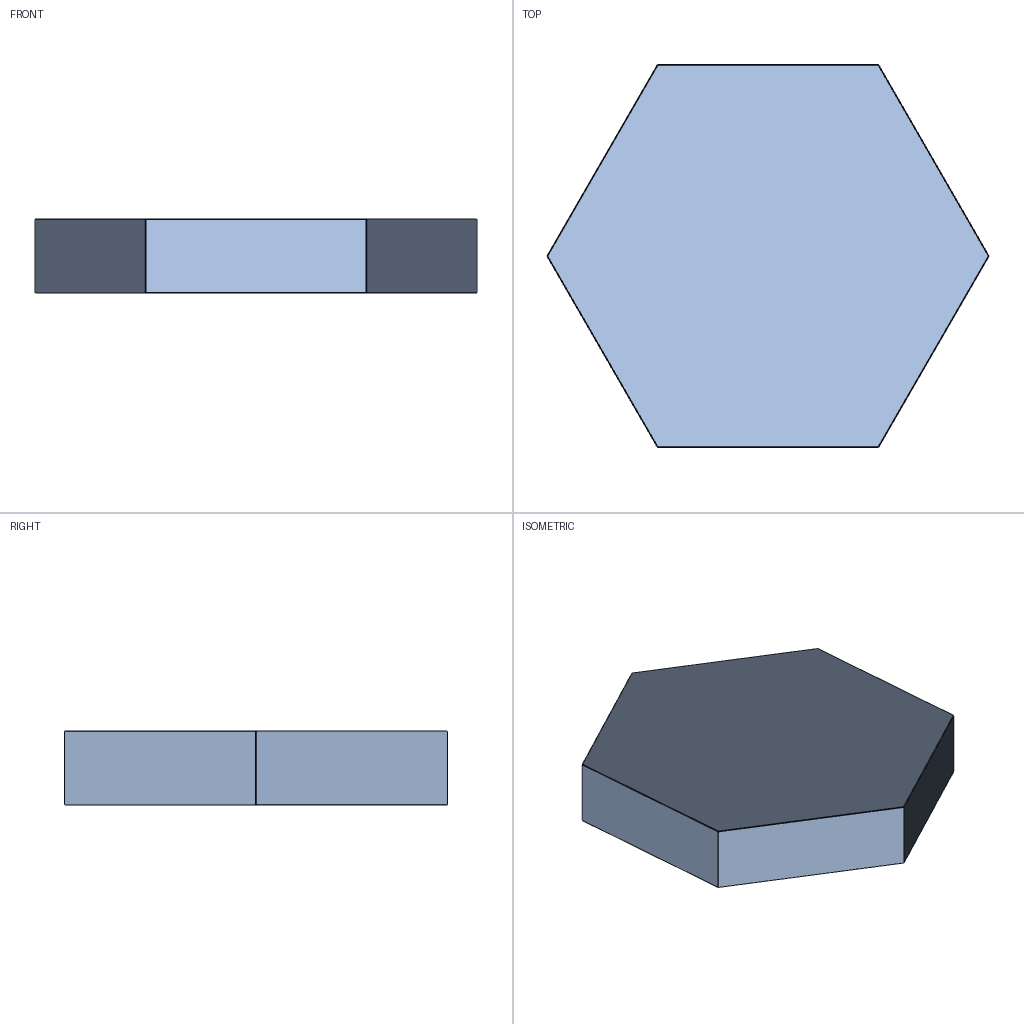
\includegraphics[width=\linewidth]{sheet_example}
\end{minipage}\hfill
\begin{minipage}[c]{0.5\textwidth}
\begin{lstlisting}[language=Python]
import cadquery as cq

r = cq.Workplane("XY")
points = [
    (0.0, 0.0974), (0.0562, 0.0), (0.1124, 0.0),
    (0.1686, 0.0), (0.2248, 0.0974), (0.1686, 0.1947),
    (0.1124, 0.1947), (0.0562, 0.1947), (0.0, 0.0974)
]
r = r.polyline(points).close()
r = r.extrude(0.0374)
\end{lstlisting}
\end{minipage}
\caption{A held-out part (\texttt{train\_high:03708}, 8 faces) and the program our model wrote for it. The prompt adds
one line of text: \texttt{Bounding box: X 0.2248, Y 0.1947, Z 0.0374}. The reference program lists six hexagon corners
and then translates the solid; ours lists nine points and skips the translation. The text differs, the solid does not
(IoU 1.000), which is why the metric executes code instead of comparing strings.}
\label{fig:task}
\end{figure}

\section{Data}

The source is CAD-Coder (Apache-2.0, derived from Text2CAD/DeepCAD): CAD parts with a written specification and a
reference CadQuery program.

\paragraph{Audit.} We executed all 82{,}659 reference programs and compared each resulting solid against the size its
own specification states. In the official \texttt{test} split, \textbf{14\% of the checkable references contradict
their own specification}; in the curated \texttt{train\_high} split, 2.3\%. Some references ignore the
specification's rotations, and some write files to disk. The benchmark is therefore drawn from \texttt{train\_high},
and the sandbox strips export calls (Section~\ref{sec:grading}).

\paragraph{Drawings sidestep the bad text.} Every sheet is rendered from the part's own reference program, so the
picture and the answer always agree even where the dataset's prose does not. Rendering uses one orthographic scale
across the three views, which is what makes elongated parts hard: the profile of a long bar occupies a few dozen
pixels.

\paragraph{Held-out rules.} The 500 benchmark parts are grouped by source part, so no benchmark part's source appears
in training (0 shared). Every training part whose geometry signature (rounded bounding-box extents and face count)
matches a benchmark part was dropped: 1{,}886 parts. Table~\ref{tab:data} lists what remains.

\begin{table}[h]
\centering\small
\begin{tabular}{lrl}
\toprule
& Parts & Notes \\
\midrule
Audited reference programs & 82{,}659 & \texttt{train\_high} 8{,}177, \texttt{train\_middle} 66{,}532, \texttt{test} 7{,}950 \\
\textbf{Benchmark (held out)} & \textbf{500} & 322 simple ($\le$6 faces), 119 medium (7--12), 59 complex ($\ge$13), 43 multi-part \\
Training, \texttt{train\_high} & 5{,}698 & remainder after removing benchmark sources and geometries \\
Training, \texttt{train\_middle} \#1 & 12{,}000 & 70\% medium/complex/multi-part \\
Training, \texttt{train\_middle} \#2 & 12{,}868 & every remaining hard part, one per geometry signature \\
\textbf{Training sheets used} & \textbf{30{,}260} & plus 306 for validation; 72\% medium/complex, 35\% multi-part \\
\bottomrule
\end{tabular}
\caption{Data inventory. Training rows are (sheet, bounding box) $\rightarrow$ reference program.}
\label{tab:data}
\end{table}

\section{Model and training}

We fine-tune \texttt{Qwen3-VL-4B-Instruct} with LoRA (rank 64, $\alpha=32$, dropout 0.05) on the language model's
projections only; the vision encoder and merger stay frozen. The loss covers the program text, never the prompt or
the image tokens. Each sheet enters at $1024\times1024$, which the processor turns into exactly 1{,}024 visual
tokens; rows are 1{,}569 tokens at the median. One epoch over 30{,}260 rows is 1{,}892 steps at an effective batch of
16, learning rate $2\times10^{-4}$ with a cosine schedule, and takes 2.9 hours on one H100 (Baseten Training). A
second epoch continues that adapter with a new data order at $1\times10^{-4}$ over four H100s (DDP, effective batch
32, 946 steps, 55 minutes) and is the model reported here; it lifts medium parts from 39.5\% to 56.3\%. Each run
ends by merging the adapter into the base weights, which vLLM then serves directly, and by grading itself on the 500
held-out sheets inside the same job.

\section{Grading}
\label{sec:grading}

A candidate program is executed in a sandbox: an import allowlist (\texttt{cadquery}, \texttt{math},
\texttt{numpy}), no dunder access, no file I/O, export calls stripped, each task in a separate process with a
timeout, run in a throwaway directory. The resulting solid is compared with the reference by exact OpenCascade
boolean volumetric IoU, maximised over the 24 axis-aligned rotations after centring, because the dataset applies its
own global transforms inconsistently. \textbf{A part counts as correct when the code runs and that aligned IoU is
$\ge0.9$}; a part 10\% too large scores 0.75 and fails. We also record IoU $\ge 0.95$, run rate, mean IoU, Chamfer
distance, latency and cost.

Rows where an API returned no answer at all (HTTP 402/5xx, dropped connections after retries) are excluded from every
score and reported separately, rather than counted as model failures. This mattered: a credit limit silently turned
32 frontier calls into 402 errors mid-benchmark.

\section{Test-time verification}

A 4B model is cheap enough to answer a part several times. To choose among candidates without an answer key, we build
each one and render it exactly as the input sheet was rendered, then score the match: the mean silhouette IoU across
the three orthographic views, multiplied by how well the candidate's bounding box matches the one given in the
prompt. On 689 real frontier answers this separates correct from incorrect with AUC 0.959, and where several answers
exist for one part it picks a correct one 98.1\% of the time (random choice: 76.3\%). Adding visible-edge matching
was measured and made it worse (AUC 0.81 alone), since the same solid built a different way has different internal
seams.

\section{Results}

Table~\ref{tab:main} and Figure~\ref{fig:tier} give the main comparison: every lane on the same 497 held-out parts,
every frontier lane at high reasoning effort and with two worked examples, ours with none.

\begin{table}[h]
\centering\small
\begin{tabular}{lrrrrrrrr}
\toprule
& All [95\% CI] & Simple & Medium & Complex & Multi & Runs & \$/1k & p50 / p95 \\
\midrule
\textbf{Ours, best of 8} & \textbf{80.7} [77--84] & \textbf{95.6} & \textbf{61.3} & \textbf{39.0} & \textbf{58.1} & 100.0 & 1.19 & 2.3 / 14.3\,s \\
\textbf{Ours, 1 sample} & \textbf{74.8} [71--79] & 92.5 & 52.1 & 25.4 & 53.5 & 99.8 & \textbf{0.22} & \textbf{2.0 / 4.4\,s} \\
GLM-5.3 Flash (high) & 66.2 [62--70] & 85.9 & 37.0 & 18.6 & 39.5 & 98.6 & 1.00 & 3.7 / 46.2\,s \\
Kimi K3 (high) & 61.8 [58--66] & 81.5 & 30.3 & 18.6 & 39.5 & 95.8 & 36.82 & 10.4 / 81.9\,s \\
Qwen3-VL-4B, untuned & 14.7 [11--18] & 19.4 & 8.4 & 1.7 & 16.3 & 34.2 & --- & 20.3 / 157.5\,s \\
\bottomrule
\end{tabular}
\caption{Correct parts (\%) on 497 held-out parts: code runs and aligned IoU $\ge 0.9$. Tiers by reference face count
(319 simple, 119 medium, 59 complex, 43 multi-part). ``Runs'' is the share of programs that build a solid. Cost is API
list price for the frontier lanes and amortised GPU price for ours (one H100, \$6.50/h, measured throughput).
Confidence intervals are bootstrap 95\%.}
\label{tab:main}
\end{table}

\begin{figure}[h]
\centering

\includegraphics[width=\textwidth]{results_by_tier}
\caption{The same numbers by part complexity, with 95\% confidence intervals. Our lead is widest exactly where the
frontier models are weakest: medium parts (61.3\% vs 37.0\%) and complex parts (39.0\% vs 18.6\%).}
\label{fig:tier}
\end{figure}

Two observations. First, a single sample already beats both frontier models while costing 4.5$\times$ less than
GLM-5.3 Flash and 167$\times$ less than Kimi K3, and it answers in 2.0\,s against 3.7\,s and 10.4\,s. Second,
best-of-8 costs about as much per part as Flash and adds 5.9 points, because the verifier recovers 96\% of what
sampling made available (its oracle, the share of parts where any of the eight was correct, is 83.7\%).

\paragraph{The verifier helps any model.} Running the frontier models with the same best-of-4 procedure on the 65
medium and complex parts lifts Kimi K3 from 27.7\% to 48.3\% and GLM-5.3 Flash from 32.3\% to 45.9\%. It is a general
technique; it is simply cheap for a 4B model and expensive for a frontier one (\$251.67 per 1{,}000 parts for K3).

\paragraph{Learning curve.} Figure~\ref{fig:curve} scores intermediate checkpoints on the same parts. The untuned
model gets 13.2\%; after 200 steps (3{,}200 examples, 11\% of the first epoch) it matches Kimi K3, it passes GLM-5.3
Flash around step 1{,}000, and the second epoch takes it to 77.0\%.

\begin{figure}[h]
\centering
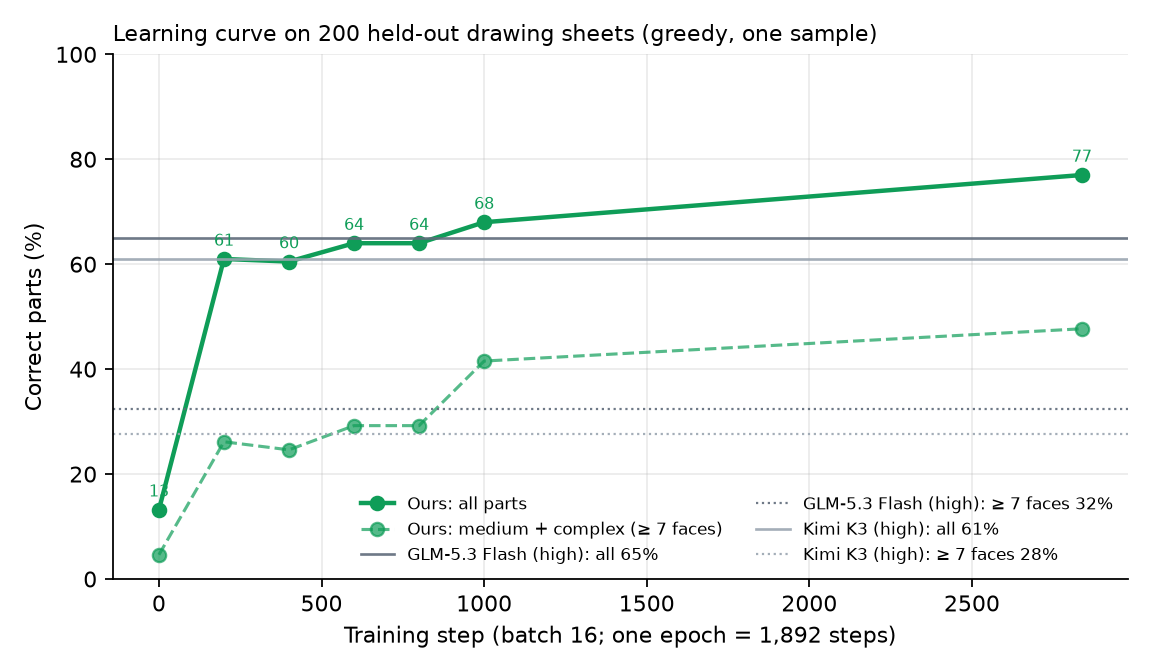
\includegraphics[width=0.85\textwidth]{learning_curve}
\caption{Accuracy against training step, all on the same 200 held-out parts, greedy decoding. Checkpoints were served
as four LoRA adapters from a single deployment and benchmarked in parallel.}
\label{fig:curve}
\end{figure}

\begin{figure}[h]
\centering

\includegraphics[width=0.62\textwidth]{cost_vs_accuracy}
\caption{Accuracy against cost per 1{,}000 parts (log scale). Our two operating points sit above and to the left of
every alternative.}
\label{fig:cost}
\end{figure}

\section{Reinforcement learning on the geometry reward did not help}

The grader is an exact, automatic reward, so the obvious next step is to optimise it directly. We ran GRPO on top of
the SFT model: 8 samples per sheet, 64 rollouts per step, 60 steps on four H100s, reward = aligned IoU, $+0.5$ when
IoU $\ge 0.9$, $-0.2$ for a program that crashes and $-0.5$ for an answer with no code in it.

It worked as an optimiser and failed as a method. Mean training reward rose from 0.89 to 1.2 and the share of correct
rollouts from 39\% to 70\%, but held-out accuracy fell. To see whether a shorter run would have helped, we graded
every saved checkpoint, and the SFT checkpoint they all start from, in a single eval-only training job that runs the
benchmark harness on each (Figure~\ref{fig:rl}). The control reproduces the SFT run's own score within two parts
(76.0\% here against the 75.6\% that run reported), so the comparison is sound.

Accuracy is already below the starting point after ten steps and never returns. The loss is almost entirely on medium
parts: 56.3\% $\rightarrow$ 48.7\% after ten steps, then flat near 42\%. Simple parts, where the model was already
right 92\% of the time, barely move, and complex parts stay inside their noise. We did not ship it.

We measured what happened but did not diagnose why, and the obvious explanation does not survive contact with the
configuration. The rollout prompts were already 80\% medium, complex or multi-part, so this is not a case of easy
prompts producing identical rewards and no gradient: the logged share of groups with zero reward variance stayed
between 0 and 0.375. What the run does show is a policy collapsing onto one mode --- entropy falls from 0.25 to 0.09
across the 60 steps --- while mean aligned IoU on held-out parts falls too, 0.887 to 0.871. So it is not trading
exactness for overlap; it gets worse at both. The reward rising while held-out accuracy falls, concentrated on the
tier with the most partial credit available, is consistent with the policy fitting the 2,000 rollout prompts rather
than the task, but we have not run the ablation that would settle it.

\begin{figure}[h]
\centering
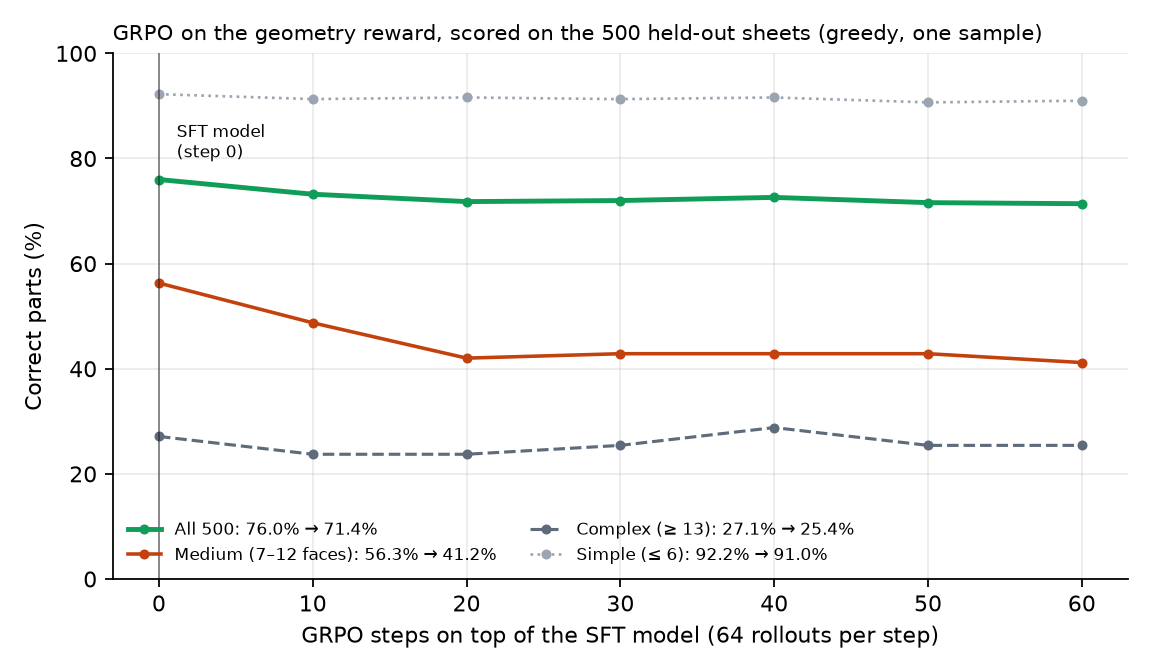
\includegraphics[width=0.78\textwidth]{rl_curve}
\caption{Every saved GRPO checkpoint, graded on the same 500 held-out sheets with the same harness as the SFT model
at step 0.}
\label{fig:rl}
\end{figure}

\section{Did it overfit, or memorise the benchmark?}

Three checks.

\paragraph{Training.} Two passes, each with its own data order. Validation loss fell monotonically to the last step of
both (epoch 1: 0.2119 $\rightarrow$ 0.1583; epoch 2: 0.1598 $\rightarrow$ 0.1490) and validation token accuracy rose
to 94.7\%, so training stopped while still improving rather than after a turn upward.

\paragraph{Exact overlap.} Zero benchmark source parts appear in training, and zero training parts share a benchmark
part's geometry signature, by construction.

\paragraph{Near-duplicates.} 57 of 500 benchmark parts have a training part within 1\% on every bounding-box axis with
the same face and part count (none within 0.1\%). Those parts are easier for every model, including ones that never
saw our data, so the question is whether \emph{our} advantage depends on them. It does not
(Table~\ref{tab:leakage}): our margin over the best frontier model is +14.9 points on the 443 parts with no
near-duplicate, slightly wider than the +14.5 overall.

\begin{table}[h]
\centering\small
\begin{tabular}{lrr}
\toprule
& Near-duplicate (57) & No near-duplicate (443) \\
\midrule
Ours, best of 8 & 94.7 & \textbf{78.8} \\
Ours, 1 sample & 94.7 & 72.2 \\
GLM-5.3 Flash (high) & 84.2 & 63.9 \\
Kimi K3 (high) & 73.7 & 60.3 \\
\bottomrule
\end{tabular}
\caption{Correct parts (\%) split by whether a near-duplicate exists in training
(\texttt{scripts/leakage\_check.py}).}
\label{tab:leakage}
\end{table}

\section{Limitations}

The model is trained and tested on one distribution: DeepCAD-style mechanical parts rendered by our own renderer.
Nothing here shows it transfers to scanned drawings, other CAD dialects, or drawings with dimension callouts instead
of a stated bounding box. The bounding box is given, which removes the global scale problem. Complex parts remain
the weak point at 39.0\%, so much of the task is still open. Finally, our cost figure assumes a busy GPU; at low
volume a per-token API is cheaper than a dedicated one.

\section{Reproducing this}

\begin{lstlisting}[language=bash]
python scripts/audit_cadcoder.py            # run every reference program, check it against its spec
python -m cadabra.cad.splits             # benchmark/training splits, held out by source part and geometry
python -m cadabra.cad.render --split bench    # drawing sheets
python -m cadabra.cad.build_vlm          # training rows + images
cd training/vlm && baseten train push --config config_vlm.py --job-name sft   # epoch 1, one H100
GPUS=4 CONTINUE_JOB=<job> CONTINUE_CHECKPOINT=checkpoint-1892 LR=1e-4 DATA_SEED=43 \
  baseten train push --config config_vlm.py --job-name sft-epoch2              # epoch 2, four H100s
./scripts/deploy_vlm.sh <job_id> H100       # merge -> vLLM on Baseten
python -m cadabra.cad.bench --modality image --lanes specialist --n 0 --shots 0 --tag ours-img
python scripts/leaderboard.py --latest sota-img,ours-img --common --out-json data/demo/scoreboard.json
python scripts/plot_results.py && python scripts/plot_curve.py && python scripts/leakage_check.py
\end{lstlisting}

Every benchmark run in the repository keeps its per-part rows, including the program each model wrote, so any number
here can be recomputed or spot-checked.

\end{document}
